NeXus is an effort by an international group of scientists to define a common data exchange and archival format for neutron, X-ray and muon experiments. NeXus is built on top of the scientific data format HDF5 and adds domain-specific rules for organizing data within HDF5 files.

\vspace{20pt}

\DTsetlength{10pt}{35pt}{5pt}{2pt}{7pt}


% \begin{figure}
% \caption{A typical nexus file layout with shape definition}
% 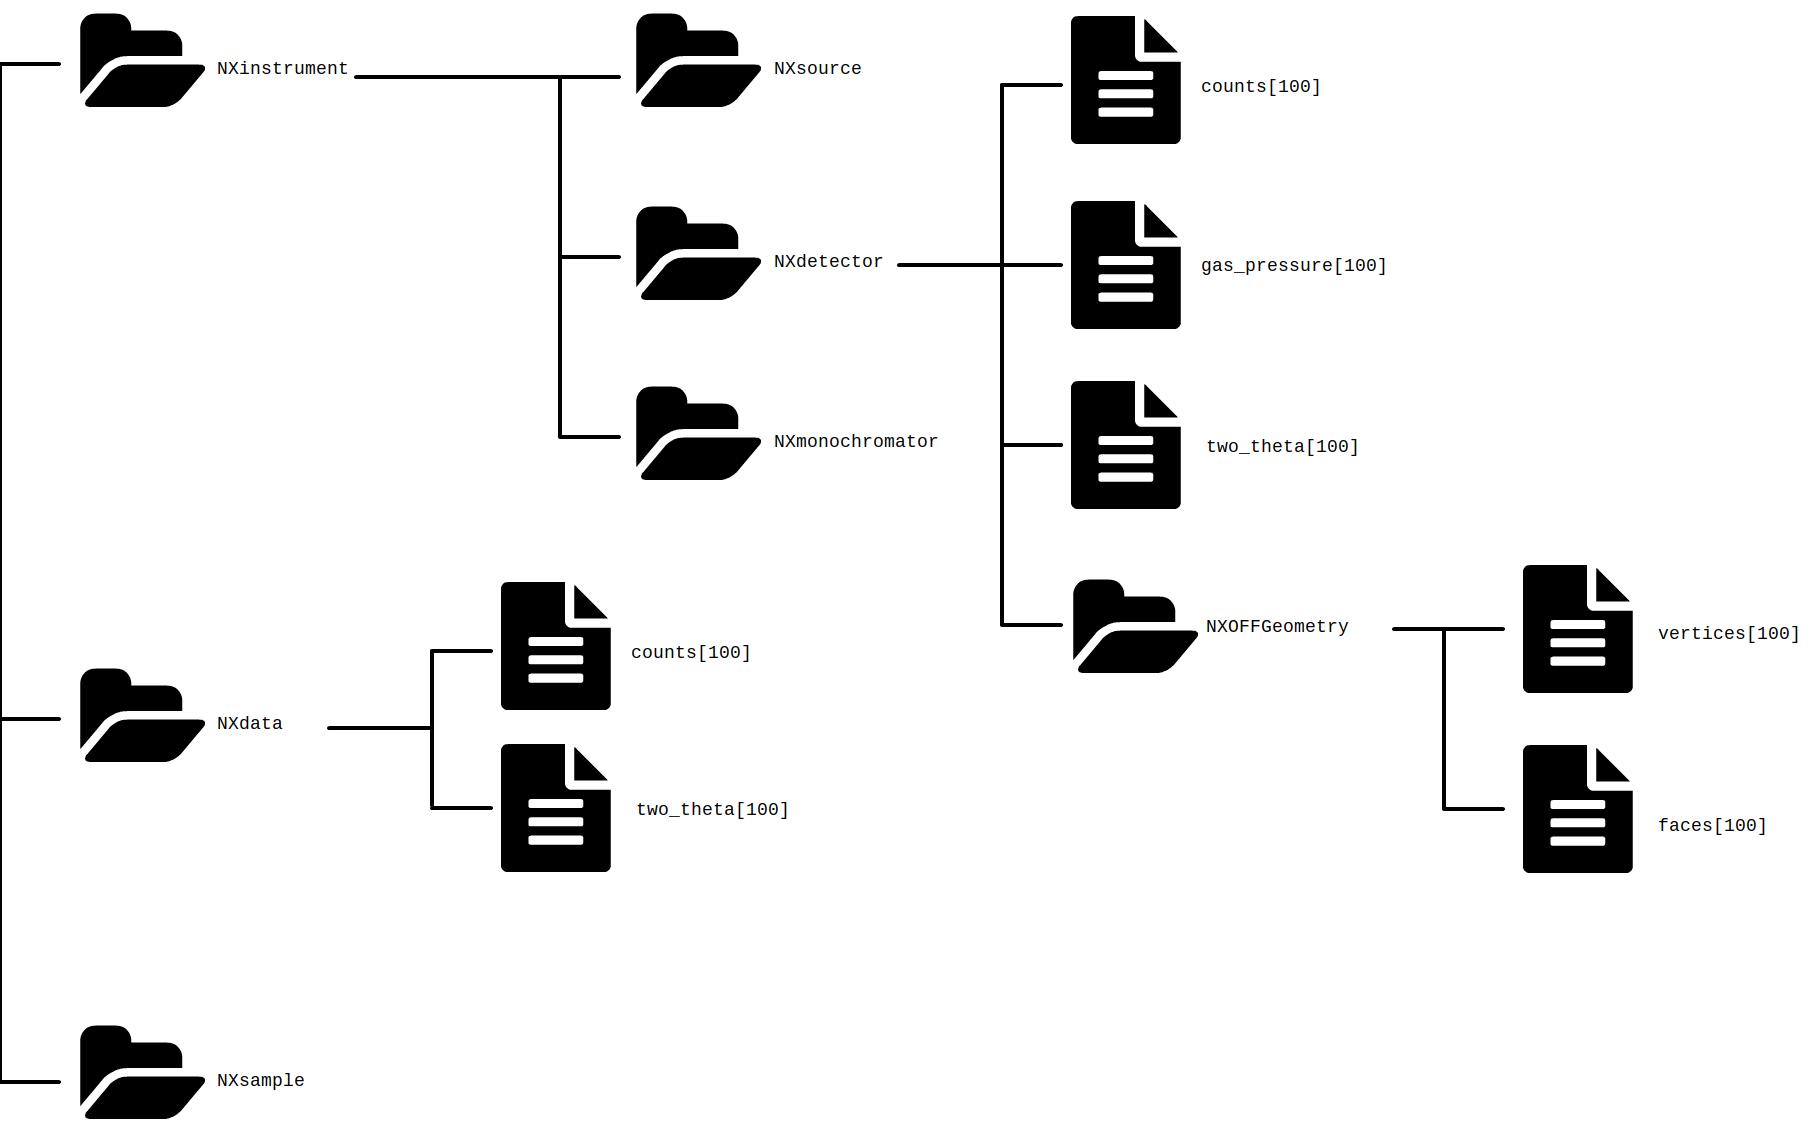
\includegraphics[width=\linewidth]{nexusdiagram.png}
\dirtree{%
.1 root.
.2 \myfolder{NXinstrument}.
.3 \myfolder{NXsource}.
.3 \myfolder{NXdetector}.
.4 \myfile{counts[100]}.
.4 \myfile{gas\_pressure[100]}.
.4 \myfile{two\_theta[100]}.
.4 \myfolder{NXoff\_geometry}.
.5 \myfile{vertices[100]}.
.5 \myfile{faces[100]}.
.3 \myfolder{NXmonochromator}.
.2 \myfolder{NXdata}.
.3 \myfile{counts[100]}.
.3 \myfile{two\_theta[100]}.
.2 \myfolder{NXsample}.
}
% \end{figure}

% What's a shape definition?

A recent addition to the NeXus standard means components that are used in experiments can specify shape definition to describe their placement, size and geometry. Transformations (NXtransformations) can be applied to these components when their position changes during or before the experiment. 
